{\color{gray}\hrule}
\begin{center}
\section{Asian Call Option Pricing}
% \textbf{You can add small descriptions of what the current sections describe}
\bigskip
\end{center}
{\color{gray}\hrule}
\begin{multicols}{2}

\subsection{Problem Statement}
An Asian call option is unique because its payoff depends on the average price of the underlying asset over a certain period, rather than just the price at maturity. \cite{PAOMCC} They are popular due to their reduced sensitivity to market manipulation and lower volatility compared to European options.

In the Black-Scholes-Merton model, this average price, \(\overline{S}_T\), is calculated as:
\[
\overline{S}_T = \frac{1}{m} \sum_{i=1}^{m} S_{t_i}\]
where:
\begin{itemize}
    \item \(t_i = i \Delta t\), 
    \item \(\Delta t = \frac{T}{m}\), 
\end{itemize}
with \(T\) being the time to maturity and \(m\) the number of time intervals.

At maturity, the payoff of the Asian call option is determined using the formula:
\[
\text{Payoff} = \max(0, \overline{S}_T - K)
\]
where \(K\) is the strike price. 

The theoretical price of the Asian call option\cite{PAOMCC} is given by:
\[
c = e^{-rT } \mathbb{E}[\max(0, \overline{S}_T - K)]
\]
where:
\begin{itemize}
    \item \(r\): the risk-free interest rate (continuously compounded),
    \item \(\mathbb{E}\): the expected value operator.
\end{itemize}

The objective of this project is to estimate the price of the Asian call option\cite{PAOBOMCC} using Monte Carlo simulation. We will evaluate how the accuracy of the method improves as the sample size \(N\) increases. The results will include:
\begin{itemize}
    \item The estimated option price,
    \item Confidence intervals,
    \item Computational time.
\end{itemize}

\subsection{Methodology}

\subsubsection{Problem Setup}

We aim to price an Asian Call option using Monte Carlo simulations under the following setup:

\begin{itemize}
    \item Spot price $(S_o) = \$100$
    \item Strike price $K = \$100 $
    \item Time to Maturity $(T)$ = 1 year
    \item Risk-free Rate $(r) = 10\%$
    \item Dividend yield $(q) = 0\%$
    \item Volatility $(\sigma) = 20\%$
    \item Number of steps $(m) = 50$
\end{itemize}

Similar to the European put option pricing problem, the convergence of the Monte Carlo method is evaluated by varying the number of simulated paths (N) and analyzing the results. We vary N by a factor of 4. This is in line with the theoretical convergence of $1/\sqrt{n}$ for Monte Carlo. By varying by a factor of 4, we aim to observe a reduction in standard error by \textbf{half}.

\subsubsection{Challenges and Considerations}

\begin{itemize}
    \item Computational Cost: The accuracy of Monte Carlo simulations improves with N, but this comes at the cost of higher computational time.
    \item Variance Reduction Techniques: Methods such as antithetic variates, control variates, or importance sampling can accelerate convergence by reducing variance. We revisit the control variate method in \ref{subsec: 3.2.3}
    \item Discretization Error: The approximation of the continuous time model with discrete time steps introduces discretization error, which can be mitigated by increasing m.
\end{itemize}

\subsubsection{Control Variate technique\cite{AOPMCCV}}
\label{subsec: 3.2.3}

The method of variance reduction using control variates works based on the underlying concept that in order to estimate a quantity from data, information about another estimator can be used to adjust the original estimator. The other estimator used as the source of information is considered the control.

For this problem, we use the geometric Asian call price as our control. We take advantage of the fact that we can calculate the analytical value of the geometric Asian call using the Black-Scholes formula. This is because the geometric average shares a key property with stock price which is the lognormal distribution.\cite{PAOBOMCC}

We define the aritmetic mean $\bar{S_A}$ and the geometric mean $\bar{S_G}$ of stock prices as,
$$
    \bar{S_A} = \frac{1}{m} \sum_{j=1}^m S(t_j)\cite{PAOBOMCC}
$$
$$
    \bar{S_G} = \frac{1}{m} \sum_{j=1}^m log(S(t_j))\cite{PAOBOMCC}
$$
Payoff of the geometric Asian call is given similar to other call options, $(\bar{S_G} - K, 0)^+$

\textbf{Black-Scholes formula for the Analytical Geometric Asian Call price}\cite{PAOBOMCC}

$G_{bs} = e^{-r^*T} \left[S(0)e^{r^*T}\cdot\phi(D1)-K\phi(D2)\right]$\cite{TBSM}

$D1 = \frac{log(S(0)/K) + (r^* + \frac{1}{2}\sigma^{*2})T}{\sigma^*\sqrt{T}}$\cite{TBSM}

$D2 = D1 - \sigma^*\sqrt{T}$\cite{TBSM}

$\sigma^* = \sigma^2 \cdot \frac{(m+1)(2m+1)}{6m^2}$\cite{TBSM}

where, $\phi(\cdot)$ is the cumulative distribution function of the standard normal distribution, $\mathcal{N}(0,1)$.

Our goal is to obtain information for our Monte Carlo estimator using the geometric prices. 

Let $C_A, C_G$ be the value of the arithmetic and geometric Asian call respectively. Let $C_{CV}$ represent the adjusted estimator. We have,
$$
    C_{CV} = C_A + \hat{a}(C_G - G_{bs})
$$
We need to find the value of $\hat{a}$ which gives us reduced variance for the same sample size. Note, irrespective of the value of $\hat{a}$, $C_CV$ is an unbiased estimator of arithmetic Asian option price as $\mathbf{E}[C_G] = G_{bs}$.

The correlation of $C_A$ and $C_G$ is observed to be very close to 1. This implies, variance can be highly reduced by assuming $\hat{a} = -1$. Therefore,
$$
    C_{CV} = C_A + (G_{bs} - C_G)
$$
% \subsubsection{Moment Matching approach}
% \text{}
\subsubsection{Moment Matching Approach}

The moment matching approach is used to reduce variance in the Monte Carlo simulations to improve the efficiency of option pricing. The idea is to adjust the simulated sample paths so that their moments (mean and variance) match the theoretical moments calculated for the underlying asset's price distribution using the Black-Scholes-Merton model. This makes sure that the simulated samples better represent the behavior of the asset price, leading to a reduction in the variability.

\textbf{Key Concept:}  
In the Black-Scholes-Merton framework, the underlying asset price (\(S_t\)) follows a lognormal distribution. The key moments of this distribution at time \(T\) are:
\begin{itemize}
    \item \textbf{Mean:} \(\mathbb{E}[S_T] = S_0 e^{(r-q)T}\),
    \item \textbf{Variance:} \(\text{Var}[S_T] = S_0^2 e^{2(r-q)T}(e^{\sigma^2 T} - 1)\).
\end{itemize}

The moment matching approach modifies the simulated asset prices so that:
\begin{itemize}
    \item The mean of the simulated prices matches \(\mathbb{E}[S_T]\),
    \item The variance of the simulated prices matches \(\text{Var}[S_T]\).
\end{itemize}

We are interested in fitting the log-normal distribution to match the moments. A log-normal distribution is a random variable whose logarithm follows a normal distribution and is characterized by its skewed shape with a fat right tail, which allows it to capture outliers better than the normal distribution. Because of such property, it is frequently used in finance to model stock prices or asset returns.

Given the first and second moments $\mathbb{E}[X]=m_1$ and $\mathbb{E}[X^2]=m_2$ of the observations, $\mu$ and $\sigma$ can be estimated\cite{chan2015moments}:

\begin{itemize}
    \item $\mu=\ln(\frac{m_1^2}{\sqrt{m2}})$
    \item $\sigma=\sqrt{\ln(\frac{m_2}{m_1^2})}$
\end{itemize}

Using the estimated {$\mu$} and {$\sigma$}, the price of Asian call ($C$) and put ($P$) can be obtained\cite{chan2015moments}:

$C=e^{\mu-rT+\frac{1}{2}\sigma^2}\Phi(\frac{\mu-\ln K + \sigma^2}{\sigma})-Ke^{-rT}\Phi(\frac{\mu-\ln K}{\sigma})$
$P=Ke^{-rT}\Phi(\frac{\ln K-\mu}{\sigma})-e^{\mu-rT+\frac{1}{2}\sigma^2}\Phi(\frac{\ln K -\mu - \sigma^2}{\sigma})$

\textbf{Application to Asian Options:}  
For Asian options, the average asset price (\(\overline{S}_T\)) is a function of multiple time steps. So, to apply moment matching:
\begin{enumerate}
    \item Simulate paths for \(S_{t_i}\) using standard Monte Carlo methods.
    \item Estimate parameters of log-normal distribution $\mu$ and $\sigma$ from the simulated stock price path.
    \item Use the estimated parameters to compute the Asian call and put option price.
\end{enumerate}
This adjustment reduced the variability in \(\overline{S}_T\), leading to more stable and accurate estimates of the option price.

\textbf{Benefits of Moment Matching:}
\begin{itemize}
    \item \textbf{Reduced Variance:} By matching the simulated samples with the true distribution, moment matching reduces noise in the simulation results.
    \item \textbf{Improved Convergence:} The estimates converge faster to the theoretical price, requiring fewer simulations to achieve a given level of accuracy.
    \item \textbf{Better Confidence Intervals:} Narrower confidence intervals indicate higher precision in the pricing results.
\end{itemize}

\subsection{Results}
While pricing the Asian call option using Monte Carlo simulations, our goal is to observe the convergence of the option price estimate, the reduction in standard error, and the tightening of confidence intervals as the number of simulated paths (N) increases. Additionally, we analyse the computational time to understand the tradeoff between accuracy and performance.
\begin{itemize}
    \item Spot price (\(S_0\)) = 100
    \item Strike price (\(K\)) = 100
    \item Time to maturity (\(T\)) = 1 year
    \item Risk-free interest rate (\(r\)) = 10\%
    \item Dividend yield (\(q\)) = 0\%
    \item Volatility (\(\sigma\)) = 20\%
    \item Number of time steps (\(m\)) = 50
\end{itemize}


\subsubsection{Convergence of Option Price}
We observe that the option price becomes stable around 7.16 as the sample size is increased. Initially, at \(N = 1,000\), the price changed significantly to 7.44726, with a larger standard error. By \(N = 256,000\), the option price converged to 7.16131, indicating improvement in the accuracy.

\subsubsection{Reduction in Standard Error}
The estimated standard error (\(SE\)) decreased consistently with larger \(N\), validating the theoretical convergence rate of \(1/\sqrt{N}\).
\begin{itemize}
    \item At \(N = 1,000\), \(SE = 0.290548\).
    \item At \(N = 4,096,000\), \(SE\) reduced to 0.00428821.
\end{itemize}

\subsubsection{Confidence Intervals}
The 95\% confidence intervals narrowed as the sample size grew, reflecting greater precision.
\begin{itemize}
    \item At \(N = 1,000\), the interval was \([6.8778, 8.01673]\), wide due to high variability.
    \item At \(N = 4,096,000\), the interval tightened to \([7.15283, 7.16964]\), indicating higher confidence in the estimate.
\end{itemize}
\end{multicols}
\begin{table}[h!]
\centering
\caption{Summary of Results for Asian Call Option Pricing}
\begin{tabular}{|p{2cm}|p{2cm}|p{2.5cm}|p{3.8cm}|p{3cm}|}
\hline
\textbf{Sample Size (\(N\))} & \textbf{Option Price} & \textbf{Estimated SE} & \textbf{95\% Confidence Interval} & \textbf{Compute Time (s)} \\ \hline
1,000      & 7.44726  & 0.290548   & [6.8778, 8.01673]   & 0.002837  \\ \hline
4,000      & 6.99283  & 0.134176   & [6.72985, 7.25581]  & 0.009831  \\ \hline
16,000     & 7.15872  & 0.0686947  & [7.02408, 7.29336]  & 0.036476  \\ \hline
64,000     & 7.16353  & 0.0341347  & [7.09663, 7.23043]  & 0.135538  \\ \hline
256,000    & 7.16131  & 0.0171805  & [7.12764, 7.19499]  & 0.514667  \\ \hline
1,024,000  & 7.15808  & 0.00858648 & [7.14125, 7.17491]  & 2.07379   \\ \hline
4,096,000  & 7.16124  & 0.00428821 & [7.15283, 7.16964]  & 7.77147   \\ \hline
\end{tabular}
\end{table}
\begin{table}[h!]
\centering
\caption{Price estimate of Various Asian Call pricing methods}
\begin{tabular}{|p{2.5cm}|p{2.5cm}|p{2.5cm}|p{2.5cm}|}
\hline
\textbf{Sample Size (\(N\))} & \textbf{Standard Method} & \textbf{Control Variate} & \textbf{Moment Matching}\\ \hline
1,000      & 7.44726  & 6.51516 & 7.89215  \\ \hline
4,000      & 6.99283  & 7.22617 & 7.80306 \\ \hline
16,000     & 7.15872  & 7.22445 & 7.84517 \\ \hline
64,000     & 7.16353  & 7.18692 & 7.7103 \\ \hline
256,000    & 7.16131  & 7.15084 & 7.72373 \\ \hline
1,024,000  & 7.15808  & 7.17222 & 7.72841 \\ \hline
4,096,000  & 7.16124  & 7.16191 & 7.7183 \\ \hline
\end{tabular}
\end{table}

\begin{multicols}{2}
\subsubsection{Computational Time}
As expected, the computational time increased with larger sample sizes. For \(N = 1,000\), the time was only 0.002837 seconds, but it rose to 7.77147 seconds at \(N = 4,096,000\). This demonstrates the tradeoff between accuracy and computational cost.

\subsubsection{Observations on Accuracy-Efficiency Tradeoff}
A sample size of \(N = 256,000\) strikes a balance between accuracy and computation time. The option price estimate at this level was 7.16131, with a standard error of 0.0171805 and a reasonably tight confidence interval. Further increasing the \(N\) provided lesser gains in accuracy but required significantly more computational resources.

\subsubsection{Comparing Methods}



While comparing methods, we observed that the standard method and the control variate approach converged to very similar values. We observed the estimate of the moment matching method varied by \$0.6. Moment matching had smaller standard errors to start with and shadowed the standard method in this regard. As you can see from the Figure 5, Control variate and the standard method converged for approximately similar values of N. This can be a good stopping point for the simulations size under computational constraints. All methods observed the theoretical convergence of $1/\sqrt{n}$ of Monte Carlo simulations without a surprise.

\subsection{Discussion}

The results for pricing the Asian call option using Monte Carlo simulations demonstrate many key insights regarding the effectiveness, accuracy, and efficiency of the standard method, control variate method, and moment matching technique. 

\subsubsection{Comparison of Pricing Methods}
\textbf{Standard Monte Carlo Method:}  
The standard Monte Carlo approach gave more accurate estimates as the sample size (\(N\)) increased, following the theoretical convergence rate of \(1 / \sqrt{N}\).  

\textbf{Accuracy vs. Computational Cost:}  
While increasing \(N\) improves accuracy, it also increases computational time. The control variate and moment matching methods provided faster convergence, offering a more efficient alternative to the standard method.

\textbf{Tradeoff Between Accuracy and Efficiency}
A key observation is that beyond a certain sample size, the improvement in accuracy becomes marginal while the computational cost increases significantly. For practical purposes, A sample size of \(N = 256,000\) strikes a good balance, further increasing \(N\) offered lesser returns in accuracy while adding a lot more computational cost.
\subsubsection{Variance Reduction Techniques}
Both the control variate and moment matching techniques demonstrated the benefits of variance reduction:
\begin{itemize}
    \item \textbf{Control Variate Method:}  
    Improved convergence without adding any significant bias, making it good for achieving high accuracy with a smaller \(N\).
    \item \textbf{Moment Matching Method:}  
    Reduced initial variability and achieved smoother predictions but added a slight upward bias to the price.
\end{itemize}

\textbf{Choice of Technique:}  
The choice of method depends on the tradeoff between computational efficiency and bias tolerance:
\begin{itemize}
    \item For applications requiring unbiased results, the control variate method is preferred.
    \item For low computational budgets and faster convergence, moment matching provides a practical alternative.
\end{itemize}

\textbf{Future Improvements:}
\begin{itemize}
    \item Implementing antithetic variates alongside control variates to further reduce variance.
    \item Exploring quasi-Monte Carlo methods (e.g., Sobol sequences) for faster convergence.
    \item Leveraging parallel computing to reduce computational time for large sample sizes.
\end{itemize}

\end{multicols}

\begin{figure}[H]
    \centering
    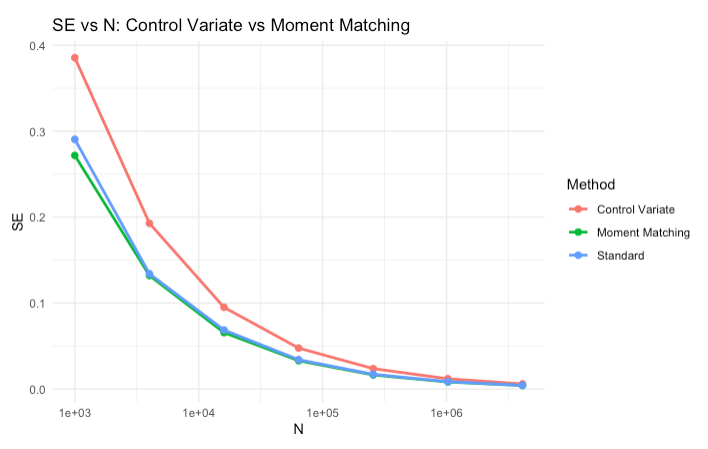
\includegraphics[width=0.9\linewidth]{se_N_comparison.png}
    \caption{Comparative plot for SE across all methods}
    \label{fig:enter-label}
\end{figure}

\begin{figure}[H]
    \centering
    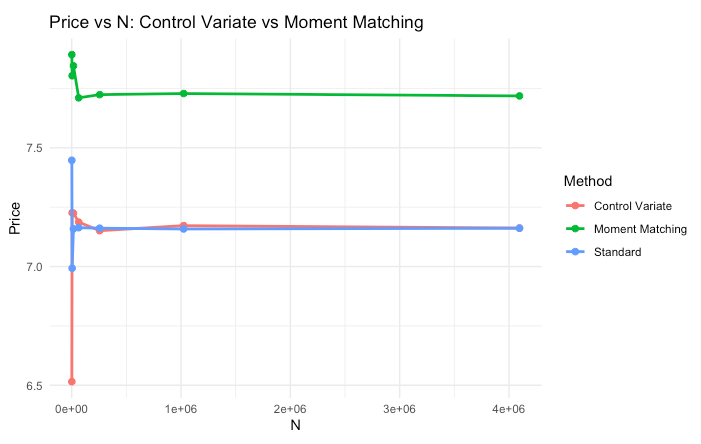
\includegraphics[width=0.9\linewidth]{price_v_N_comparison.png}
    \caption{Comparative plot for Price across all methods}
    \label{fig:enter-label}
\end{figure}